\documentclass{article}
\usepackage{tikz}
\usetikzlibrary{arrows.meta,positioning,calc,shapes.geometric}
\pagestyle{empty}
\begin{document}
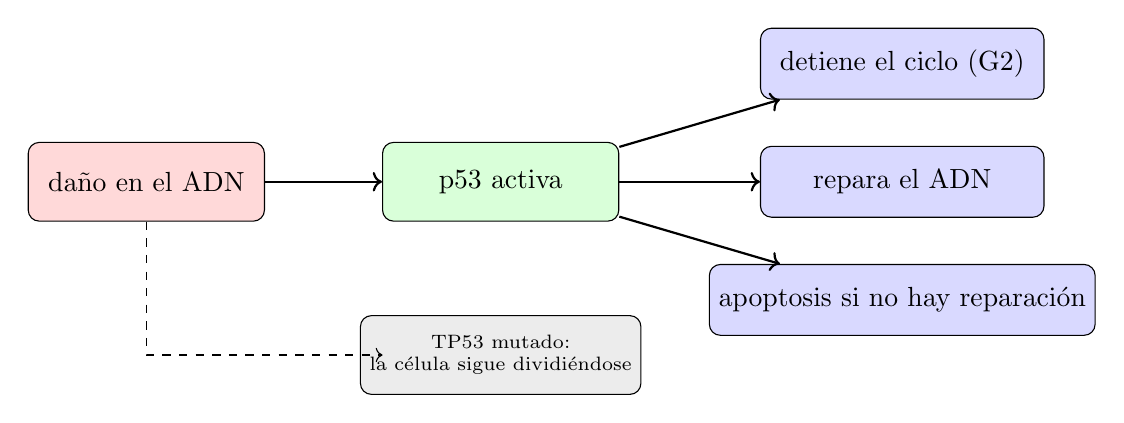
\begin{tikzpicture}
\tikzset{every node/.append style={align=center}}

\node[draw, rounded corners, fill=red!15, minimum width=3cm, minimum height=1cm, align=center] (d) at (0,0) {daño en el ADN};
\node[draw, rounded corners, fill=green!15, minimum width=3cm, minimum height=1cm, align=center] (p) at (4.5,0) {p53 activa};
\node[draw, rounded corners, fill=blue!15, minimum width=3.6cm, minimum height=0.9cm, align=center] (a) at (9.6,1.5) {detiene el ciclo (G2)};
\node[draw, rounded corners, fill=blue!15, minimum width=3.6cm, minimum height=0.9cm, align=center] (r) at (9.6,0) {repara el ADN};
\node[draw, rounded corners, fill=blue!15, minimum width=3.6cm, minimum height=0.9cm, align=center] (m) at (9.6,-1.5) {apoptosis si no hay reparación};
\draw[->, thick] (d) -- (p); \draw[->, thick] (p) -- (a); \draw[->, thick] (p) -- (r); \draw[->, thick] (p) -- (m);
\node[draw, rounded corners, fill=gray!15, minimum width=3cm, minimum height=1cm, align=center, font=\scriptsize] at (4.5,-2.2) {TP53 mutado:\\ la célula sigue dividiéndose};
\draw[->, dashed] (d) |- (3.0,-2.2);

\end{tikzpicture}
\end{document}
